\documentclass[12pt,a4paper]{article}
\usepackage[utf8]{inputenc}
\usepackage[T1]{fontenc}
\usepackage[utf8]{inputenc}
\usepackage[french]{babel}
\usepackage{graphicx}
\usepackage[T1]{fontenc}
\usepackage{graphicx}
\usepackage{caption}





\begin{document}

\begin{center}

\section*{Introduction}
\end{center}
  YouTube  est un site web d'hébergement de vidéos et média social sur lequel les utilisateurs ont la possibilité d'envoyer, regarder, commenter, évaluer et partager des vidéos en streaming.le machine learning est un domaine d'investigation consacré à la compréhension et 
à la construction de méthodes qui «apprennent», c'est-à-dire des méthodes qui exploitent les données pour améliorer les performances sur un ensemble de tâches. Ainsi,Les 
révolutions scientifiques sont toujours inspirées de la nature humaine, qu'elles soient physique ou intellectuelle. Ainsi quelle place occupe le Machine Learning dans le système de recommandation de YouTube? Et comment fonctionne le système de recommandation
de YouTube? Répondre à ces questions fera l'objet de notre étude. 
\newpage
\section{Le Machine Learning dans le système de recommandation}
 Nous pouvons effectuer différentes activités sur YouTube et nous remarquons aussi qu'au cour de ses 12 dernières années, les algorithmes ont beaucoup variées\cite{mckelvey2022portee}. Lorsque nous effectuons des recherches sur YouTube, Automatiquement YouTube nous recommande et propose des résultats,  et nous  suggère en fonction de notre recherche , Les recommandations sont celles capables de de nous plaire ou de nous apporter satisfaction à une recherche. Nous distinguons suite à une recherche des recommandations selon les cas suivants d'après YouTube Belgique : notre recherche, analyse des données, présentations, vidéos similaires, la source,les vidéos mis en ligne récemment, les vidéos regardées précédemment. Ainsi dans la figure ci dessous nous avons l'interface de YouTube après la recherche d'une vidéos et les éléments recommandés à droite dans la section à suivre.
 
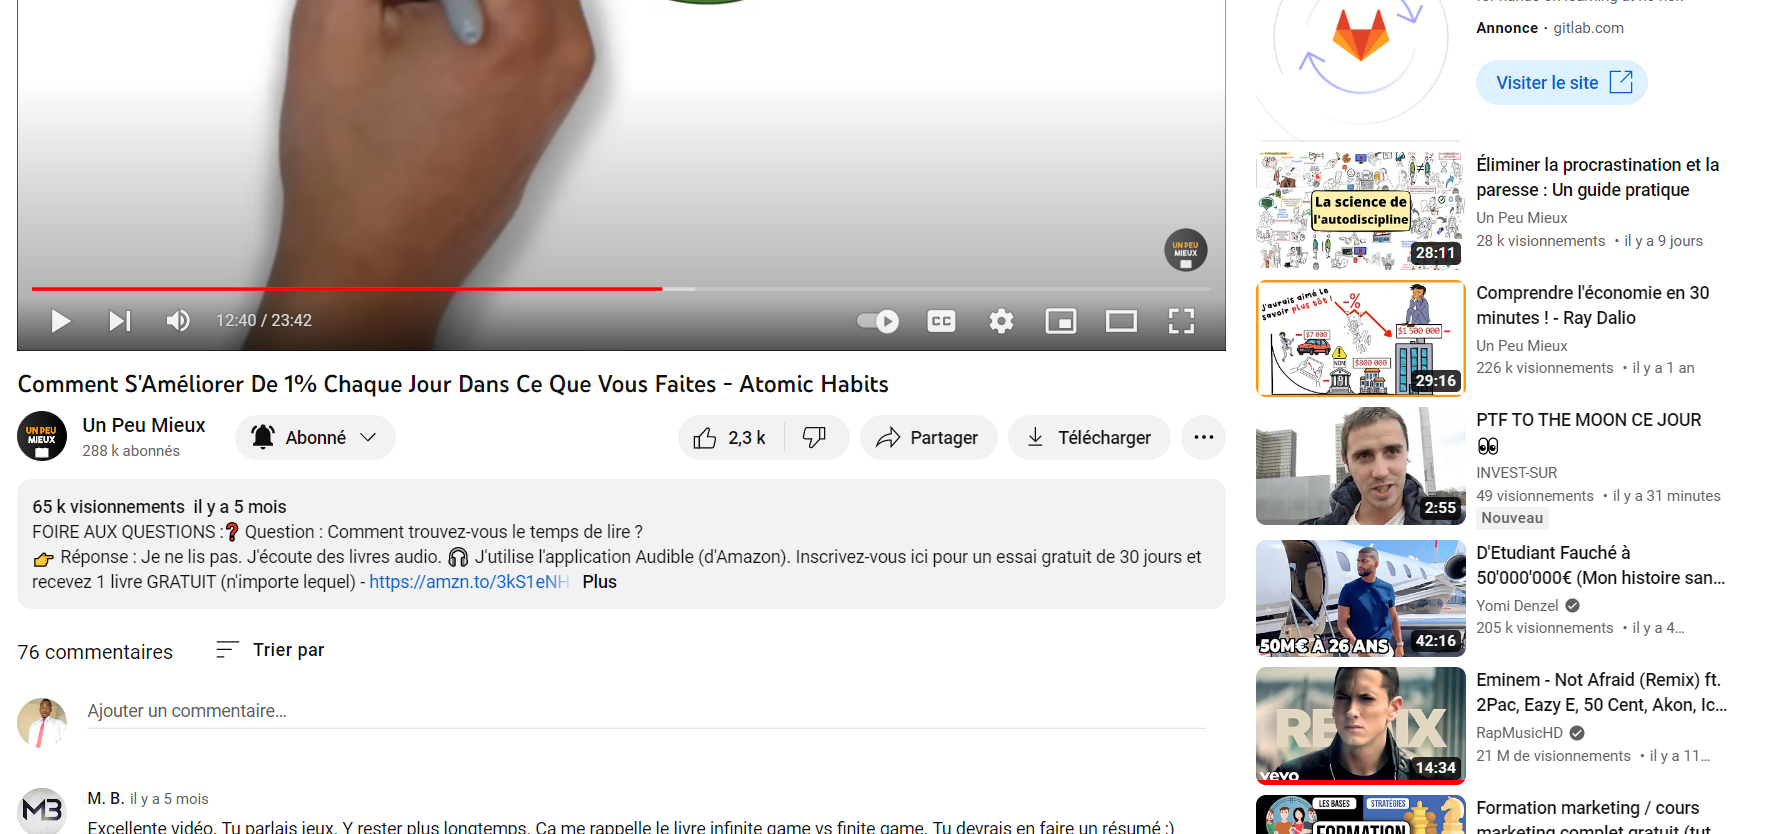
\includegraphics[width=1.1\linewidth]{Capture 9}
\captionof{figure}{Interface de youtube avec videos recommande a la suite d'une lecture}


\section{Les différentes approche du systèmes de recommandation }	

Nous distinguons plusieurs approches dans le système de recommandation  donc nous pouvons citer : l'approche basé sur le contenu, l'approche basé sur le filtrage collaboratif, l'approche hybride,l'approche basée sur la mémoire, l'approche base sur le modèle, la factorisation des matrices et le deep learning. 

\includegraphics[width=1\linewidth]{Capture 3}
\captionof{figure}{Les différentes approches du système de recommandation}


 
\section{Approche base sur le contenu}	
 une approche basé sur le contenu consiste a repérer les éléments qui correspondent le mieux avec les préférences de l'utilisateur. Cette technique se focalise sur les caractéristiques des produits afin de recommander aux utilisateurs les produits qui auront de nouvelles propriétés 
similaire avec des produits avec lesquels ils ont déjà interagit; Il s'agit du contenu similaire avec celui que j'ai aimé.Une telle approche ne requiert pas une grande communauté d’utilisateurs ou un gros historique d'utilisation du système. La figure 2 illustre ce processus.

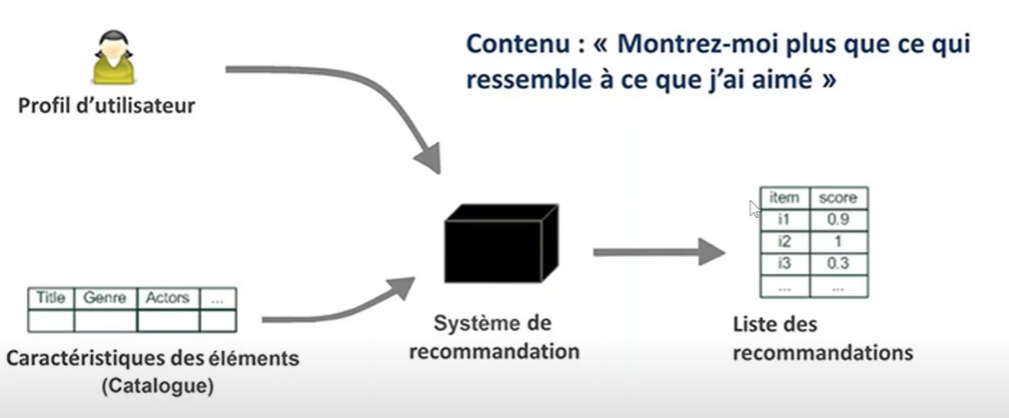
\includegraphics[width=1.1\linewidth]{Capture 1}
\captionof{figure}{ Un système de recommandation basé sur le contenu (adapté de [JZFF10]).}



Ici, il cherche à établir des profils descriptifs des utilisateurs puis à comparer ces profils aux données rencontrées pendant leurs navigation. L'hypothèse de travail est : "L'utilisateur x aime les items présentant les caractéristiques {c1,...cn}, Nous pouvons lui recommander des items présentant les mêmes caractéristiques. Le profil de l'utilisateur est exprimé sous forme d’une liste d’intérêts basée sur les mêmes caractéristiques. La coïncidence entre les caractéristiques des éléments et le profil de l'utilisateur peut être mesurée de différentes manières :l’indice de Dice ou d’autres mesures de similarité [BYRN99],
le TF-IDF (Term Frequency-Inverse Document Frequency) [SWY75],
les techniques basées sur la similarité des espaces vectoriels (les approches bayésiennes [PB07], les arbres de décision, etc.) couplées avec des techniques statistiques, lorsqu’il y a trop de mots-clés.Pour avoir des recommandation,nous pouvons utiliser une matrice; ensuite on calcule pour chaque paire item-item les similarité sur la base de vecteurs. on peut calculer cette similarité grace aux formules telles que le coefficient de corrélation Pearson ou la similarité cosinus. 


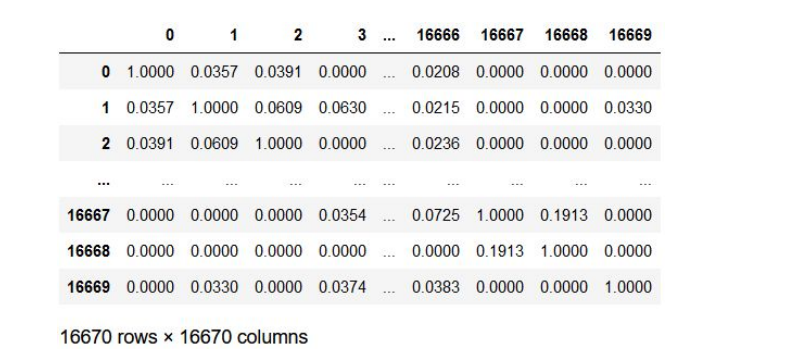
\includegraphics[width=1\linewidth]{Capture 4}
\captionof{figure}{Matrices de similarités calculée sur r 16670 items. Chaque case représente la similarité cosinus calculée d’une paire item-item. La diagonale représente les items comparés avec eux-mêmes, d’où une similarité parfaite de 1. }




\section{Approche basée sur le filtrage collaboratif }	
Une approche basée sur le filtrage collaboratif produisent des recommandations en calculant la similarité entre les préférences d'un utilisateur et d'autres utilisateurs. Cette méthode s'appuie sur l'information relative aux utilisateurs pour calculer la similarité entre deux produits utilisateurs.

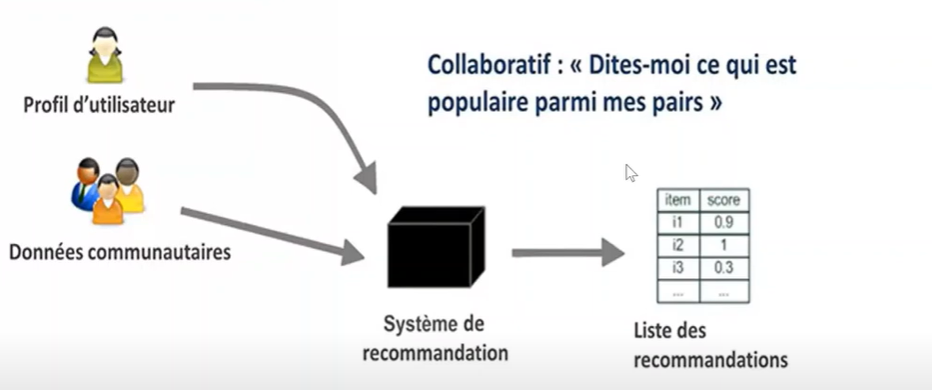
\includegraphics[width=1\linewidth]{Capture2}
\captionof{figure}{Un système de recommandation collaboratif (adapté de [JZFF10]). }




 Ici le Systeme de recommandation cherche a croiser les navigations des utilisateurs pour faire profiter les uns des liens entre donnees recoltees sur les autres. La liason entre un item et un utilisateur se fait sur la base de l'hypothese suivante : "les utilisateurs qui ont aimé les memes items que l'utilisateur x aiment aussi ces items la que nous pouvons recommander a x'".
 
 \subsection{Collecte de données}
 Directe : Par l'évaluation directe de l'utilisateur. La nous avons une evalution de l'utilisateur des vidéos auxquels il a apporté un avis
 
Indirecte :Données obtenues par l'évaluation indirecte de l'utilisateur . Ici le systeme de recommandation observe si l'utilisateur a observe si l'utilisateur a regardé une video entièrement,à moitié ou quelques minutes. En fonction de ses différents crictères on peut collecter les données sur une données.

\subsection{User-To-User}
Les recommandations sont faites en trouvant des utilisateurs ayant des avis similaire. En exemple nous pouvons énumérer : "Bidias et Paul aiment tous les deux l'item 2 et n'aime pas l'Item 3, il semble qu'ils ont des avis similaire, ce qui suggère qu'en général Bidias et Paul sont du même avis. Donc l'Item1 est une bonne recommandation pour Paul
\subsection{Iterm-To-Iterm}
Les recommandations sont faites en trouvant les items qui ont le même intérêt par plusieurs utilisateurs. Ricardo et Sandra aime L'Item 1 et L'Item 4. cela suggère qu'en général, les utilisateurs qui aiment l'Item 4 aimerons aussi L'item 1.Ainsi ,L'item 1 Pourra être recommande a Tim. 
\section{Approche hybride}
L'approche hybride utilisent de différents types d'approche de recommandation ou s'appuie sur la leurs logique. Par exemple un tel système peut utiliser a la fois des connaissances extérieures et les caractéristiques des éléments combinant ainsi des approches collaboratives basées sur le contenu.


\section{Approche basée sur la mémoire}
 Nous pouvons evoquer ici \cite{Bastin2021} dans cette méthode L'approche basée sur la mémoire utilise les interactions passées des utilisateurs pour
calculer les similitudes entre ceux-ci ou entre les items. Pour trouver la note r qu'un
utilisateur u donnerait à un item i , l'approche recherche les utilisateurs similaires à u
qui ont noté l’item i et calcule la note r en fonction des notes des utilisateurs trouvés à
l'étape précédente. Afin de trouver les U utilisateurs les plus similaires à l'utilisateur u ,
on calcule la similarité sur base des items communément notés avec l'utilisateur comparé
en calculant leur distance ou leur similarité.\\ 
NB : Notez que deux utilisateurs A et B peuvent être considérés comme
absolument similaires dans la métrique de similarité cosinus malgré des
évaluations différentes. Un exemple serait un utilisateur critique de cinéma qui attribue toujours des notes inférieures à la moyenne, mais dont le classement des éléments de sa liste serait similaire à celui des évaluateurs moyens comme B. Pour tenir compte de ces préférences individuelles des utilisateurs, il faut amener tous les utilisateurs au même niveau en supprimant leurs préjugés. Ceci peut se faire en
soustrayant la note moyenne donnée par cet utilisateur à tous les items de chaque item noté par cet utilisateur.\\
NB : Notez que deux utilisateurs A et B peuvent être considérés comme
absolument similaires dans la métrique de similarité cosinus malgré des
évaluations différentes. Un exemple serait un utilisateur critique de cinéma qui attribue toujours des notes inférieures à la moyenne, mais dont le classement des éléments de sa liste serait similaire à celui des évaluateurs moyens comme B. Pour tenir compte de ces préférences individuelles des utilisateurs, il faut amener tous les utilisateurs au même niveau en supprimant leurs préjugés. Ceci peut se faire en soustrayant la note moyenne donnée par cet utilisateur à tous les items de chaque item noté par cet utilisateur.Après avoir déterminé une liste d'utilisateurs similaire à un utilisateur u, on calcule la note r que u donnerait à un certain item i .
On considère que la note r d'un utilisateur pour un item i sera proche de la moyenne des
notes attribuées à i par les U utilisateurs les plus similaires à u . La formule mathématique de la note moyenne donnée par U utilisateurs se calcule avec formule dont la version la plus simple est :

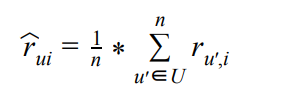
\includegraphics[width=0.8\linewidth]{Capture 5}
\captionof{figure}{r représente la note donnée par un utilisateur u à un ite, i et U représente le groupe d'utilisateur similaire a u. }
Il est également possible de multiplier la note par le degré de similarité entre les deux utilisateurs afin de donner plus de poids aux notes d'utilisateurs fort similaires à u :
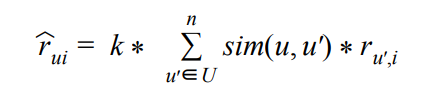
\includegraphics[width=1\linewidth]{Capture 6}
\captionof{figure}{k est un facteur de normalisation. }
Enfin, on peut également prendre en compte les notes moyennes de l'utilisateur u dans le calcul étant donné que les utilisateurs peuvent avoir tendance à voter différemment les uns des autres :
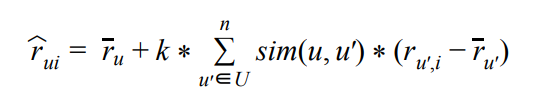
\includegraphics[width=1\linewidth]{Capture 7}
\captionof{figure}{ru est la moyenne des notes de l'utilisateur  u pour tout les items notes par u. }

	
\section{Système de recommandation d'après notre recherche}
Ici ,En fonction de notre recherche , YouTube peut nous recommander des vidéos similaire à notre
recherche. Alors ce qui va se passer dans ce cas c'est que l'algorithme va utiliser les différents termes(expressions) de notre recherche et aller
dans la base de données rechercher les éléments similaires. Et lorsque nous Postons une vidéo sous youTube nous mettons les différents mots 
susceptibles de retrouver notre vidéos. Figueiredo et ses collaborateurs (Figueiredo et al., 2014) ont, par
exemple, comparé un échantillon de vidéos les plus populaires sur
YouTube et un échantillon de vidéos aléatoire. Pour les vidéos de
l’échantillon de vidéos populaires, les vues provenant de la
recommandation algorithmique sont plus importantes. Nous pouvons évoquer ici
\cite{benbouzid2020cadran} l'auteur stipule que <<Dans le domaine des études sur YouTube, on trouve deux approches
différentes traitant du système de recommandation : d'une part, l'analyse de la contribution de la recommandation à la popularité des
vidéos et, d'autre part, l'audit des mécanismes de filtrage algorithmique
des contenus recommandés aux usagers, notamment en matière de
radicalisation politique. >>  

\section{Le système de recommandation en mode Streaming }
Le streaming est un type de technologie multimédia qui fournit du contenu vidéo et audio à un appareil connecté à Internet. Cela nous permet d'accéder à du contenu (TV, films, musique, podcasts) à tout moment, sur un ordinateur ou un appareil mobile, sans tenir compte d'une horaire de diffusion. c'est ainsi que de puissant algorithmes sont définit lors du streaming. Nous avons l'exemple \cite{beuscart2019algorithmes} ou l'auteur dit <<Pour guider l'usager dans ce catalogue, les services proposent une variété d'outils algorithmiques suggérant ou choisissant des titres : depuis l'outil de
filtrage collaboratif (« les gens qui ont aimé ce titre que vous avez écouté ont
aussi aimé celui-ci »), de recommandation thématique (« les autres titres de
cet artiste, de ce sous-genre du hip-hop que vous avez écouté ») jusqu'aux
radios thématiques (« radio inspirée de cet artiste ») ou aux playlists complètement « inspirées de vos goûts » (le « flow » de Deezer, les « découvertes de
la semaine » de Spotify), en passant par les nombreuses « ambiances » mises
en playlists pour s'adapter aux humeurs des usagers.>> Page 3. Nous remarquerons aussi dans de nombreux pays que YouTube est la plateforme la plus utilisées par les jeunes c'est ainsi que d'après un sondage ,\cite{wiard2019qui} YouTube serait la plus utilisée au sein des jeunes. 


\section{Les systèmes de recommandation basée sur le deep learning }

 Le deep learning ou apprentissage profond regroupe les méthodes d'apprentissage
automatique tentant de modéliser avec un haut niveau d'abstraction des données grâce à
des transformations non linéaires. La recommandation YouTube aide beaucoup dans la recherche de nos différents sujets ( Musique, vidéos ,documentaires et autres ) ainsi suite à des termes entrees en recherche, Le système de recommandation va alors interroger la base de données et nous renvoyer tous les éléments capable de nous intéresser et cela en liaison avec notre nos différents mots insere dans la barre de recherche. Elle s'appuie sur l'évolution de la neurosciences. c'est que \cite{covington2016deep} affirme que : <<Les systèmes d'apprentissage automatique présentent souvent un biais implicite vers le passé parce qu'ils sont entraînés à prédire l'avenir comportement à partir d'exemples historiques. >> Ainsi pour mieux comprendre YouTube dans nous allons étudier le papier blanc publiée en 2016 par YouTube expliquant leur approche du problème (Deep Neural Networks for YouTube
Recommendations). Recommander du nouveau contenu pour YouTube n'est pas une tâche
simple, le site est le deuxième site web le plus visité aux États-Unis, avec plus de 500 heures de contenu téléchargé par minute (Statista, mai 2019). YouTube a beaucoup fait
évoluer son algorithme depuis lors, mais ce papier reste un exemple concret de la manière dont on peut utiliser le deep learning par rapport aux techniques que nous avons utilisées jusqu'à présent. Ainsi nous distinguons 02 facteurs de recommandation chez YouTube 
-

\section{Les problèmes liés aux  systèmes de recommandation }
Le système de recommandation rencontre parfois des difficultés de recommandations car nous avons des utilisateurs qui ne crée pas de compte utilisateur, ne renseigne aucune donnée. Alors, le systeme fournie pour ces personnes les contenus les plus populaires et les plus vues en recommandation.  Nous avons aussi YouTube qui est associe a certains problèmes et d'aou il proneraient certains contenus nous avons le cas de \cite{tufekci2018youtube} ou l'auteur met en exergue le critique qui a été fait a YouTube Selon une théorie ou la plateforme ferait la promotion d'une theorie de complot et les recommandations conduiraient a un réseau de 9000 vidéos.

\begin{center}
\newpage
\section*{Conclusion}
\end{center}
Le machine learning permet a YouTube d'améliorer sa capacité à analyser et synchroniser les différentes recommandations suites à des recherches ou des visites. Ainsi grâce aux données enregistres par l'ordinateur, celui-ci est capable de mieux renseigner les prochains utilisateurs ou nous fournir un contenu adapte a notre recherche. ainsi , lorsque les recommandations de YouTube fonctionnent bien, elles relient des milliards de personnes dans le monde à des contenus qui les inspirent, leur enseignent des choses et les divertissent.

 
\newpage
\bibliographystyle{plain}
\bibliography{biblio.bib}
\end{document}
